\documentclass[a4paper,12pt]{article}
\usepackage{graphicx}

\usepackage{booktabs}

\begin{document}
	\title{Student Scorecard}
	\author{Kaustav Ghosh}
	\date{\today}
	\maketitle
	
	
	\begin{figure}[t!]
		\flushright
		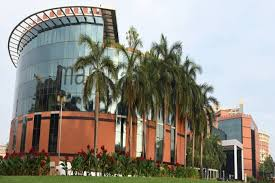
\includegraphics[height=0.5cm]{manipal.jpg}
	\end{figure}
	
	\begin{table}[ht!]
		\centering
			\begin{tabular}{c|c|c}
			Subject & Marks & Grade\\
			\hline
			Physics & 90 & B\\
			\hline
			Chemistry & 91 & A\\
			\hline
			Maths & 92 & A\\
			\hline
			English & 93 & A+\\
			\hline
			Total & 376 & Gpa = 9.78\\
			\cline{1-2}
			Cgpa & 9.99 & Class 12\\
			\hline
			\end{tabular}
	\end{table}


	\begin{table}[b!]
		\centering
		\begin{tabular}{lcr}
		Student  & CCC  & HOD \\
		 Signature &  Signature &  Signature\\
		\hline
		\end{tabular}
	\end{table}



\end{document}

